\documentclass{article}

 % Dans le préambule
%\usepackage[style=author]{biblatex} % package de bibliographie, on cite l’auteur
%\addbibresource{Bib2Validation.bib} % notre fichier bib exporté

%%%%% Tous les packages
\usepackage[left=2cm,right=2cm,top=2cm,bottom=2cm]{geometry}
\usepackage[utf8]{inputenc}% accents in
\usepackage[english]{babel}% typo française
\usepackage[T1]{fontenc}% accents out
\usepackage{lmodern}
\usepackage{titlepic}
\usepackage[noae]{Sweave} % "noae" permet à Sweave de reconnaitre les guillemets
\usepackage[%
    all,
    defaultlines=3 % nombre minimum de lignes
]{nowidow} % éviter les lignes orphelines

% package maths
\usepackage{amsmath}
\usepackage{amsfonts}
\usepackage{amssymb}
\usepackage{ dsfont } %proba
\usepackage{ stmaryrd }
% tables et figures
	
\usepackage{subfigure}
\usepackage{lscape}
\usepackage{multirow} % permet de fusionner les colonnes
\usepackage{graphicx} % admet les figures
\usepackage{array} % types particuliers de tableaux
\usepackage{tabularx} % autres tableaux, notamment pour gérer les doubles traits de séparation (voir hhline)
\usepackage{listings} % pas forcément utile ici, mais permet de faire des box avec du code
\usepackage[hang,font = normalsize, labelfont=bf,textfont=bf]{caption} % mise en forme du caption
% hyperlinks
\usepackage{hyperref}
\hypersetup{ %moduler les couleurs des liens
    colorlinks=true,
    linkcolor=black,
    % filecolor=magenta,      
    urlcolor= blue,
}
\usepackage{indentfirst} % Pour indenter les premiers paragraphes de section
%kableExtra
\usepackage{booktabs}
\usepackage{longtable}
\usepackage{array}
\usepackage{multirow}
\usepackage{wrapfig}
\usepackage{float}
\usepackage{colortbl}
\usepackage{pdflscape}
\usepackage{tabu}
\usepackage{threeparttable}
\usepackage{threeparttablex}
\usepackage[normalem]{ulem}
\usepackage{makecell}
\usepackage{xcolor}
\usepackage{hyperref} %pour les liens url
%\usepackage[absolute,overlay]{textpos}

% Pour ne pas que la mention "Chapter" apparaisse à chaque chapitre mais juste le titre du chapitre
\usepackage{titlesec}
\titleformat{\chapter}{\normalfont\LARGE}{\thechapter.}{30pt}{\LARGE\bf}
\titleformat{\section}
  {\normalfont\fontsize{15}{15}\bfseries}{\thesection}{1em}{}
\titlespacing*{\chapter}{0pt}{1.1\baselineskip}{\baselineskip}



% Ne pas sauter de page entre deux chapitres





% titres
\title{\centering 

\vspace{1 cm}

{\begin{minipage}\linewidth
        \centering
     \textbf{Un effet inattendu du confinement : une chute de la surmortalité violente chez les jeunes ?} \\[1 cm] 
        \vspace{0.5cm}
        \large Abel Aussant, Eliot Forcadell et Ariane Sessego\\
         M2 Quantifier en Sciences Sociales\\
        \vspace{0.5cm}
         \textit{Identification causale} Cours d'Olivier Godechot \\
         Année académique 2021-2022\\
    \end{minipage}}
  }
\date{}
%box

\begin{document}
\Sconcordance{concordance:Aussant_Forcadell_Sessego.tex:Aussant_Forcadell_Sessego.Rnw:%
1 116 1 1 19 31 1 1 16 3 1 1 10 1 7 55 1}

\maketitle

\cleardoublepage%

En 2020, les épisodes de confinements ont bouleversé la vie des Français. Ces restrictions de sortie en dehors du domicile avaient pour but de protéger les plus vulnérables du virus de la Covid-19, particulièrement les personnes âgées. Mais on peut se demander s'ils n'ont pas aussi eu des effets inattendus : le confinement a-t-il entrainé une diminution de la mortalité chez les jeunes ? \\

En effet, le risque de décès entre 15 et 30 ans est souvent plus élevé que l'on ne pourrait s'y attendre face à l'augmentation exponentielle de la mortalité habituellement constatée entre 10 et 60 ans (Remund, Camarada, 2021). On désigne donc comme "surmortalité" cet excès par rapport au risque de décès attendu, qui a longtemps été considéré comme uniquement masculin, lié aux turbulences hormonales et de développement biologiques des jeunes hommes\footnote{Heligman L., Pollard J.H., The age pattern of mortality, Journal of the Institute of Actuaries, 1980, 107(1), p. 49-80 et  Goldstein J. A., Secular trend toward earlier male sexual maturity: Evidence from shifting ages of male young adult mortality, PLoS ONE, 2011, 6(8), e14826.}, et liée à des causes violentes de décès (accidents, homicides...). Ces théories développementalistes ont été largement remises en question, du fait des variations de cette tendance dans le temps et l'espace ; cette surmortalité semble avant tout liée à des contexte socio-historiques particulier (Remund, Camarada, 2021). En France aujourd'hui, bien qu'elle touche aussi les jeunes femmes, cette surmortalité est bien plus importante parmi les hommes, avec en moyenne trois fois plus de décès masculins que féminin à ces âges (Breton, Barbieri, 2018). Elle est avant tout caractérisée par une part importante d'accidents de la circulation et de morts violentes (autres types d'accidents, homicides ou suicides) qui sont l'origine de 80\% des décès à ces âges (Remund, Camarada, 2021, trouver une ref plus récente parce parle des années 1960). \\

Le confinement a théoriquement réduit l'exposition à ces risques, à l'exception du suicide. A-t-il entraîné une diminution de la mortalité au sein de cette population ? Le deuxième confinement, moins restrictif que le premier, a-t-il eu un impact plus faible sur cette mortalité ? \\

La méthode de différence de différence (DD) offre la possibilité de comparer la mortalité des jeunes adultes avant et pendant les périodes de confinement en prenant en compte la saisonnalité de la mortalité et une éventuelle variation de mortalité propre à 2020. En effet, il s'agit ici d'évaluer l'effet d'un "traitement" - le confinement généralisé de la population - sur le groupe traité - les jeunes adultes. En l'absence d'expérience aléatoire, nous ne disposons pas de groupe contrôle, et toute la population étant supposée confinée, il semble difficile d'en construire un. Mais nous pouvons procéder autrement pour construire un contrefactuel, notamment en considérant les périodes précédentes. Cela suppose que l’évolution de la mortalité dans la population cible (les jeunes adultes) est comparable entre période. Or, on sait que la mortalité connait des tendances saisonnières importantes : la mortalité des jeunes adultes, en particulier, connait deux pics annuels, l'un en hiver (en février particulièrement), qui suit la tendance générale de la population, l'autre en été (en juillet), qui est lié à une augmentation estivale de mortalité par accidents (Breton, 2019). Ces tendances nous empêche de comparer simplement la période pré-confinement à la période de confinement. La DD nous permet, en supposant que l'évolution de la mortalité est comparable d'une année sur l'autre, de comparer la mortalité en 2020 (groupe traité) et pendant les années précédentes (groupe contrôle), avant les confinements (période précédent le traitement) et durant chaque confinement (période de traitement), afin de mettre en avant un eventuel effet causal du confinement sur la mortalité des jeunes adultes en France en 2020. \\

Après une présentation des données et quelques analyses descriptives, nous présenterons en détail les modèles choisis, pour ensuite commenter les résultats.

\section{Données et méthode}






\section{Données}

Pour ce faire, nous utilisons les données d'état civil mises à disposition par l'INSEE, répertoriant les personnes décédées par date de décès, année de naissance, sexe, et lieu de décès pour les années 2014 à 2020 (INSEE 2014 à 2020, voir la section \ref{source} \textit{infra}). Nous disposons du jour, du mois et de l'année de décès pour 2018 à 2020, mais uniquement du mois et de l'année de décès pour 2014 à 2017.








Concentrons nous tout d'abord sur les années 2018 à 2020, car ce sont les seuls années pour lesquelles nous disposons des décès par jour. 












\subsection{Quelques statistiques descriptives}


Nombre de décès moyen par jour 2018-2019-2020 (environ 10,4 décès par jour), déviation standard (environ 3,5)
Il faut juste que je mette en forme les données


\begin{center}
\begin{figure}[h!]
\caption{\label{Graph_descr}Tendances mortalité par jour (gaussian smoothing)}
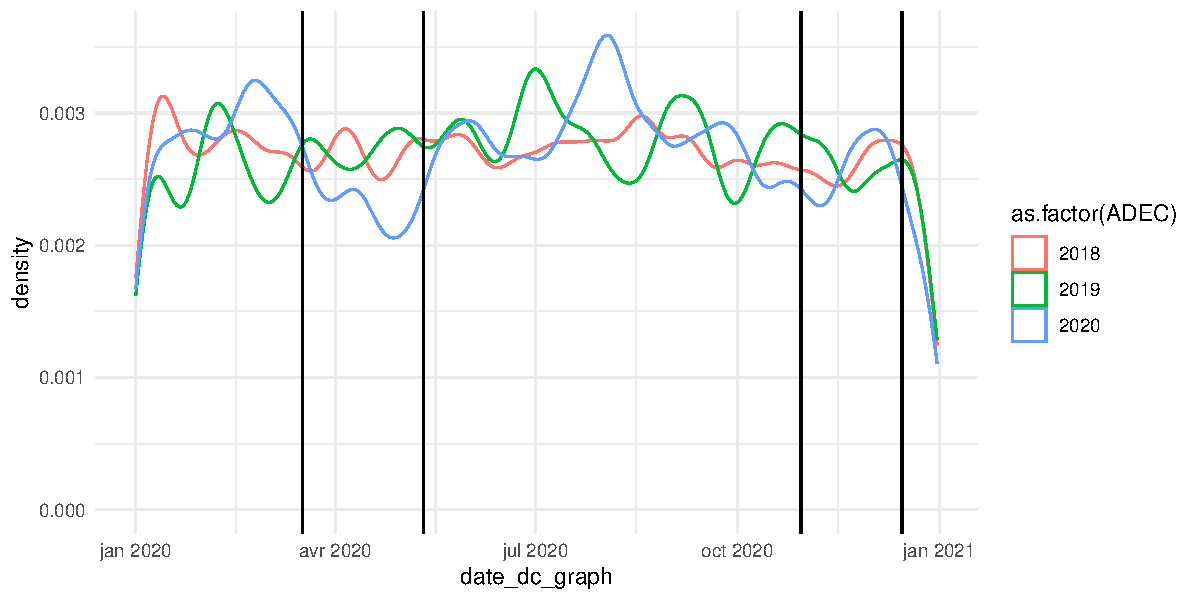
\includegraphics{Aussant_Forcadell_Sessego-003}
\end{figure}
\end{center}








\section{Résultats}

\subsection{La méthode de différence de différence et les régressions choisies}


\subsection{Les modèles de régressions choisies}

Comparer les périodes de confinements aux tendances de début d'années (on suppose que les jeunes sont peu touchés par le Covid, et que les trends du milieu d'année sont touchées par un effet Covid)\\

- Ajouter un effet année \\

- Ajouter un effet weekend \\

- Se demander si la diminution de la mortalité pendant le confinement n'est pas contrebalancée par une augmentation de la mortalité post-confinement ? (il semblerait que pas totalement)\\





\section{Résultats et Discussion}

Régressions \\


Limites : \\

- Les faibles effectifs font que les tendances sont assez chaotiques, il faudrait comparer sur plus longtemps. \\

- Trop peu d'effectifs pour comparer homme/femme. \\



\section{Sources} \label{source}

\begin{itemize}
\item INSEE, 2020, \url{https://www.insee.fr/fr/statistiques/5431034?sommaire=5419788&q=d\%C3\%A9c\%C3\%A8s+2020}
\item INSEE, 2019, \url{https://www.insee.fr/fr/statistiques/4801913?sommaire=4768339&q=d\%C3\%A9c\%C3\%A8s+2019}
\item INSEE, 2018, \url{https://www.insee.fr/fr/statistiques/4216603?sommaire=4215184}
\item INSEE, 2017, \url{https://www.insee.fr/fr/statistiques/3606190?sommaire=3596198}
\item INSEE, 2016, \url{https://www.insee.fr/fr/statistiques/3053349?sommaire=3051496}
\item INSEE, 2015, \url{https://www.insee.fr/fr/statistiques/2406453?sommaire=2406457}
\item INSEE, 2014, \url{https://www.insee.fr/fr/statistiques/2114975?sommaire=2114983}
\end{itemize}


\end{document}
